\begin{figure}[htp]
  \centering
  \subfloat[$WZ$ ROC curve in \zdom{} training]{
    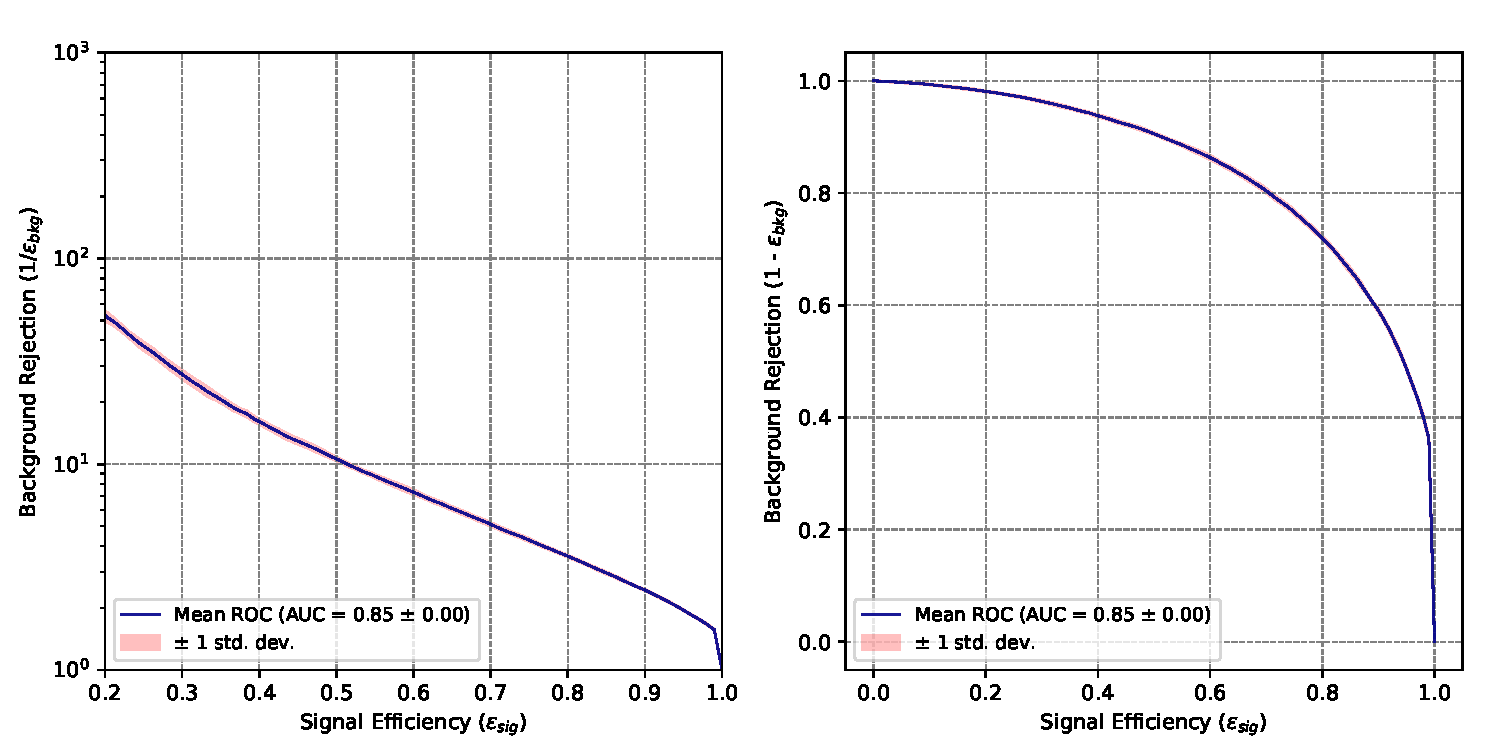
\includegraphics[width=0.8\textwidth]{figures/VH/VH_kfold_roc_wz_zdom.pdf}\label{fig:vh_wz_zdom_roc}
  }
  \hfill
  \subfloat[$ZZ$ ROC curve in \zdom{} training]{
    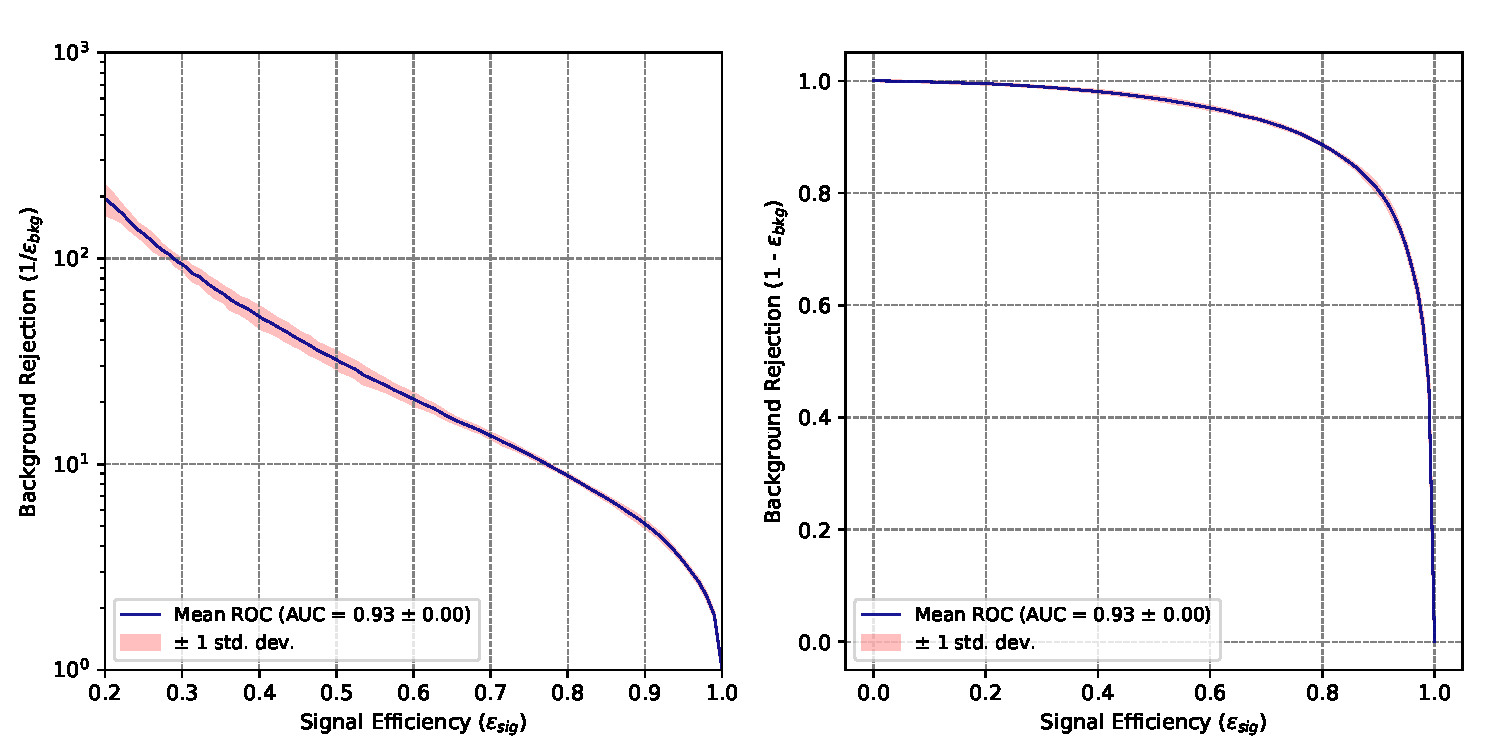
\includegraphics[width=0.8\textwidth]{figures/VH/VH_kfold_roc_zz_zdom.pdf}\label{fig:vh_zz_zdom_roc}
  }
  \hfill
  \subfloat[$WH$ vs All ROC curve in \zdom{} training]{
    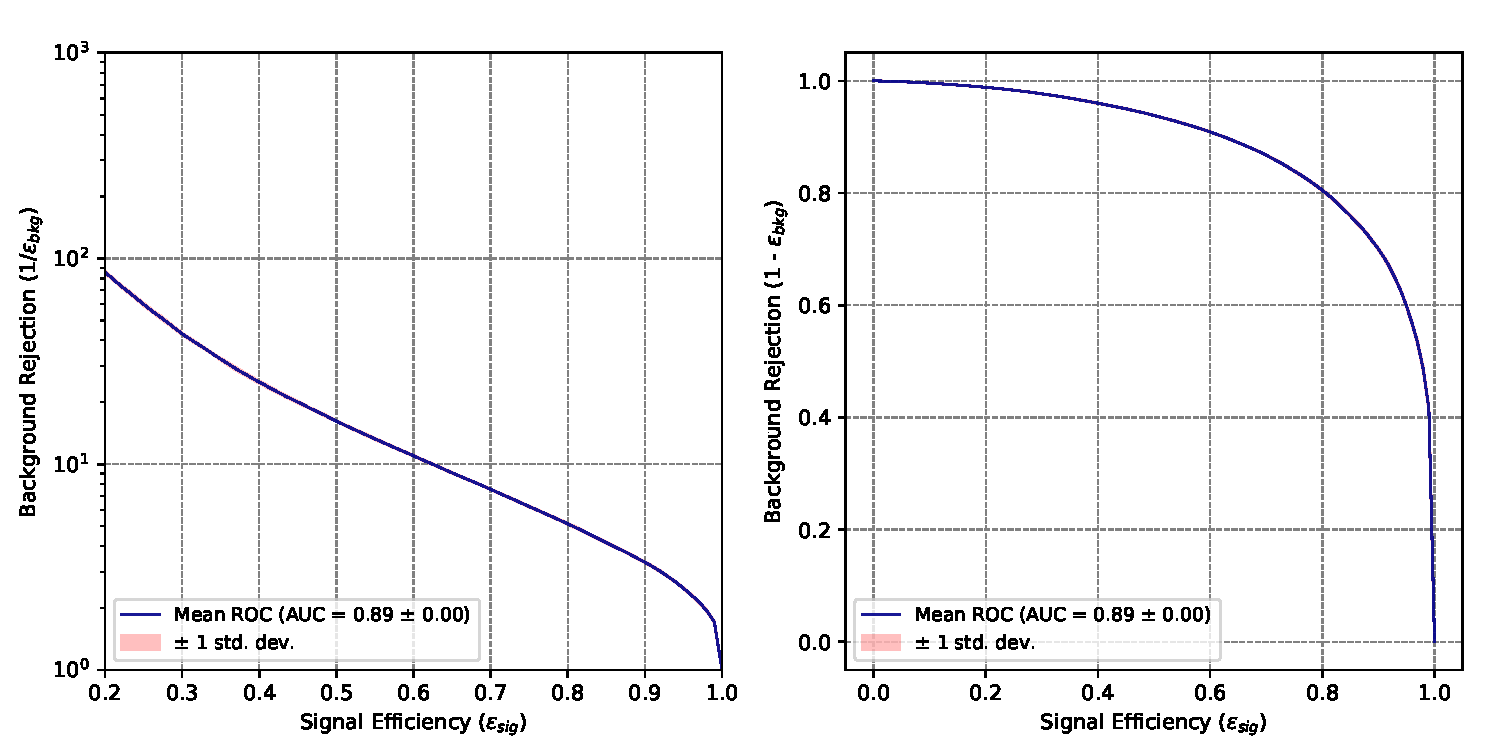
\includegraphics[width=0.8\textwidth]{figures/VH/VH_kfold_roc_ova_zdom.pdf}\label{fig:vh_ova_zdom_roc}
  }
  \caption{ROC curves for the ANN performance in the \zdom{} SR\@. The curves are averaged over the five folds of the cross-validation, with the shaded area representing the standard deviation across folds. The curves demonstrate good performance due to the high area under the curve (AUC) score.}\label{fig:vh_wh_zdom_roc}
\end{figure}

\begin{figure}[htp]
  \centering
  \subfloat[$WZ$ ROC curve in \zdom{} training]{
    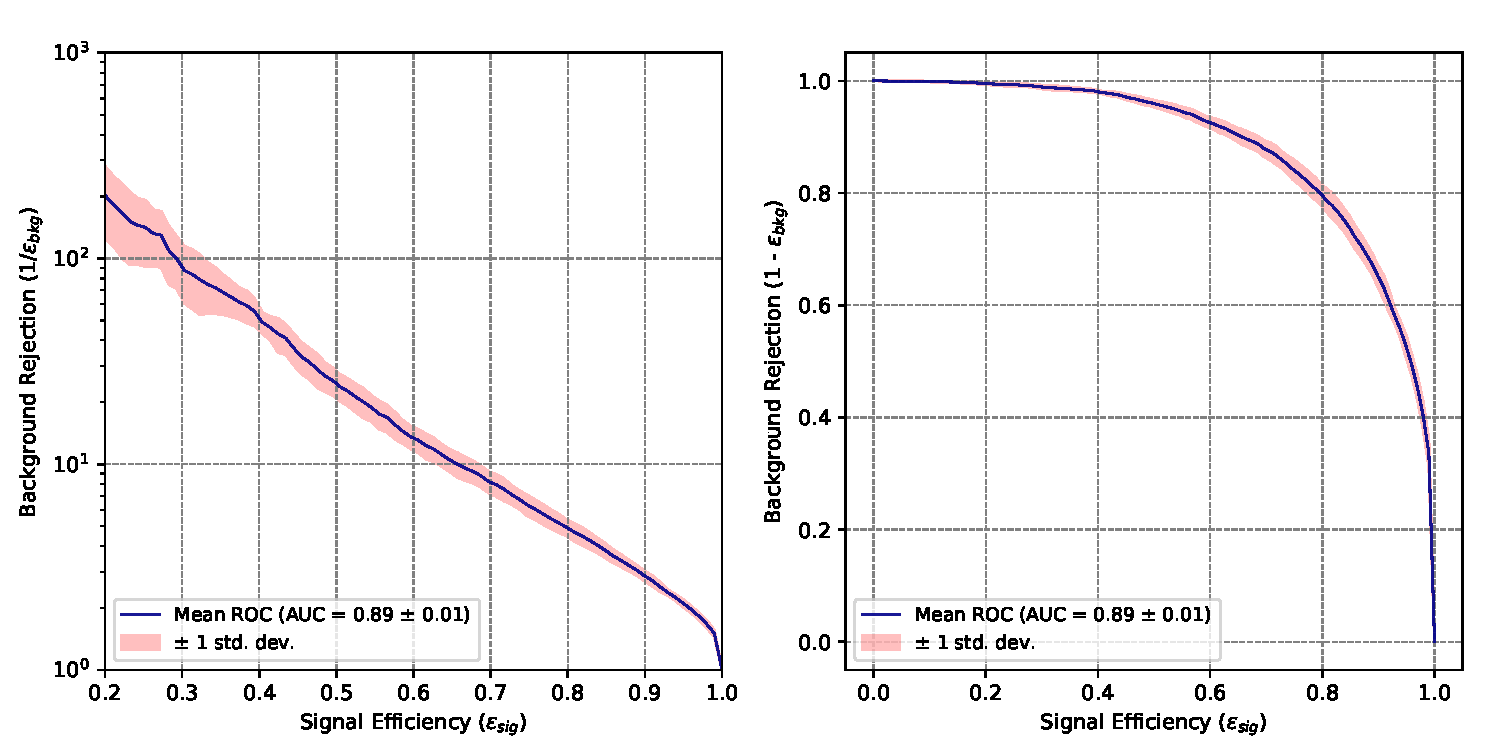
\includegraphics[width=0.6\textwidth]{figures/VH/VH_kfold_roc_wz_zdep.pdf}\label{fig:vh_wz_zdep_roc}
  }
  \hfill
  \subfloat[$WWW$ ROC curve in \zdom{} training]{
    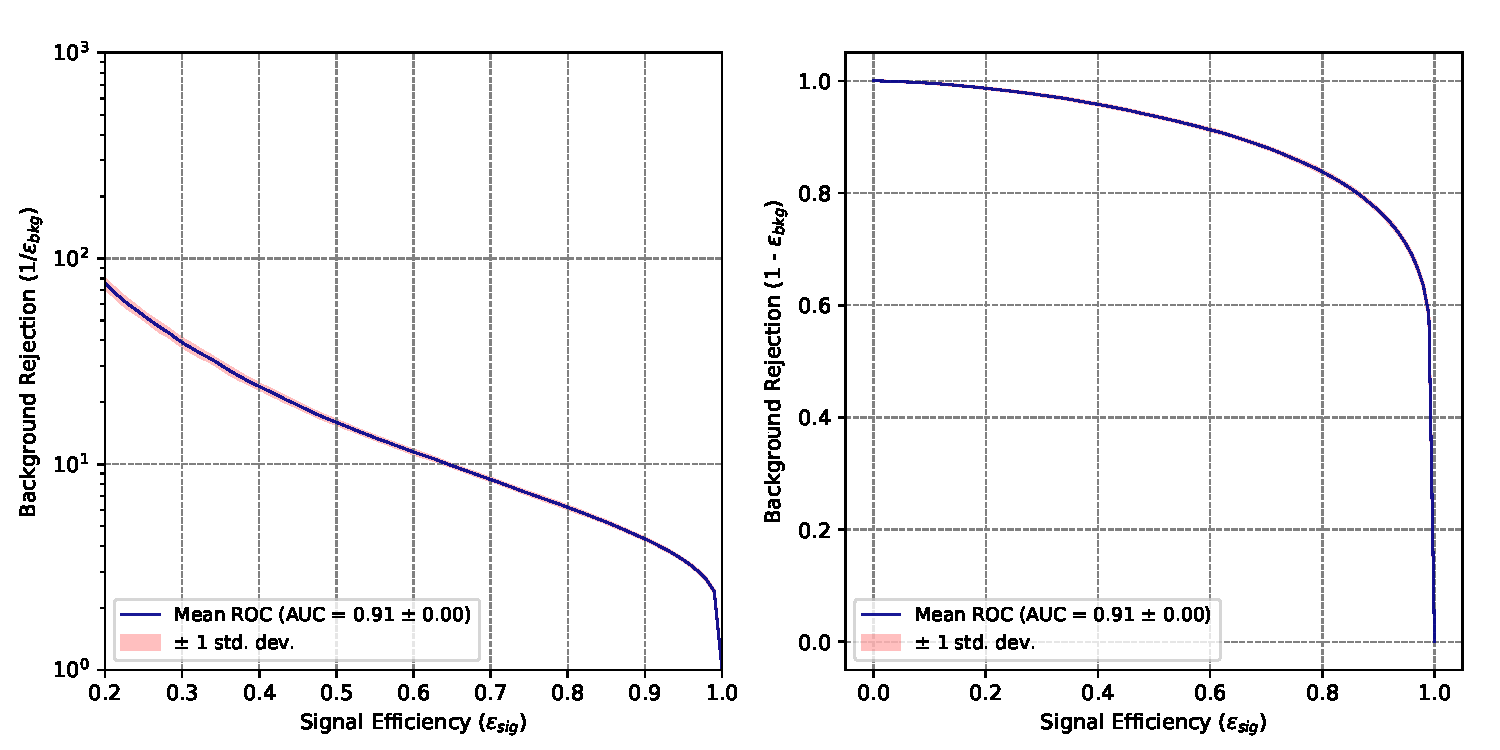
\includegraphics[width=0.6\textwidth]{figures/VH/VH_kfold_roc_www_zdep.pdf}\label{fig:vh_www_zdep_roc}
  }
  \hfill
  \subfloat[$t\bar{t}$ ROC curve in \zdom{} training]{
    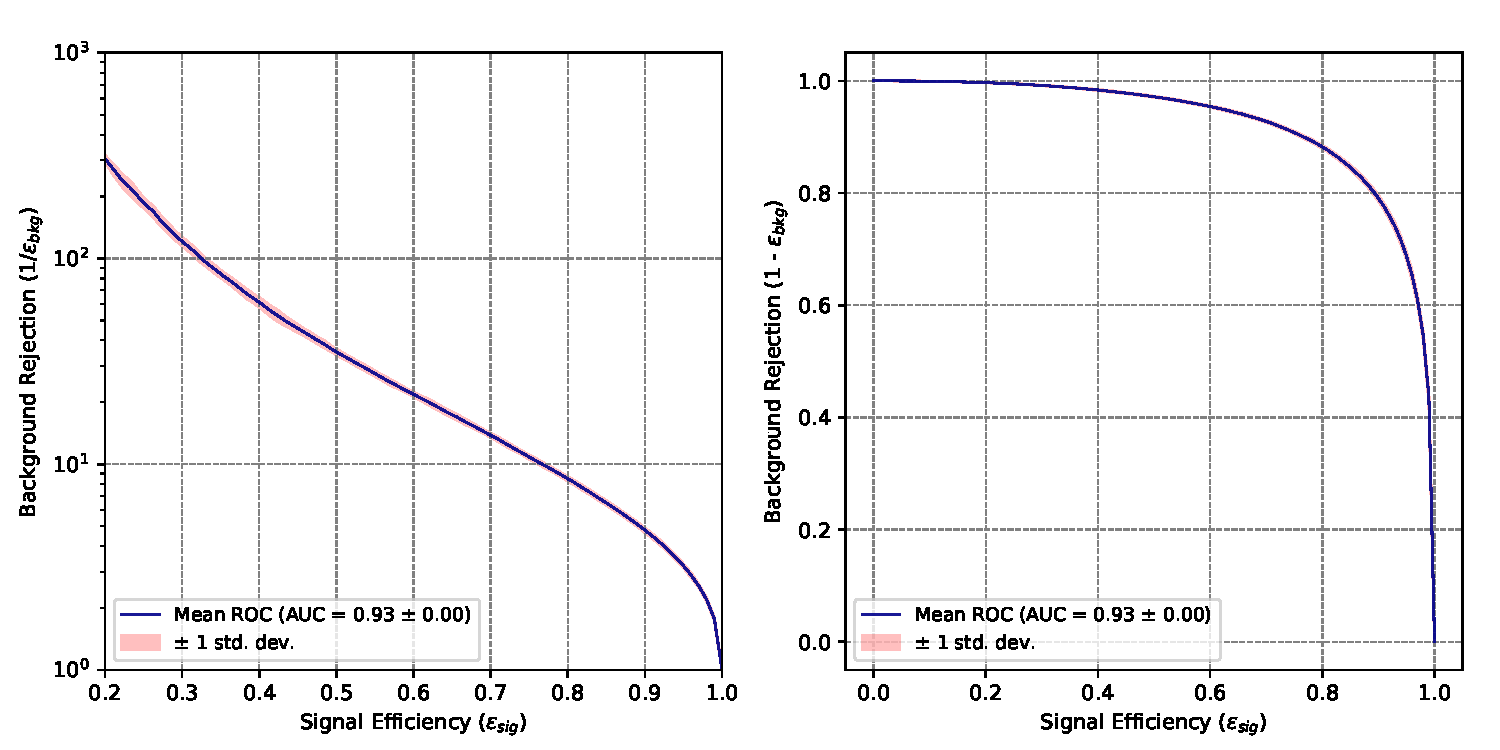
\includegraphics[width=0.6\textwidth]{figures/VH/VH_kfold_roc_ttbar_zdep.pdf}\label{fig:vh_ttbar_zdom_roc}
  }
  \hfill
  \subfloat[$WH$ vs All ROC curve in \zdom{} training]{
    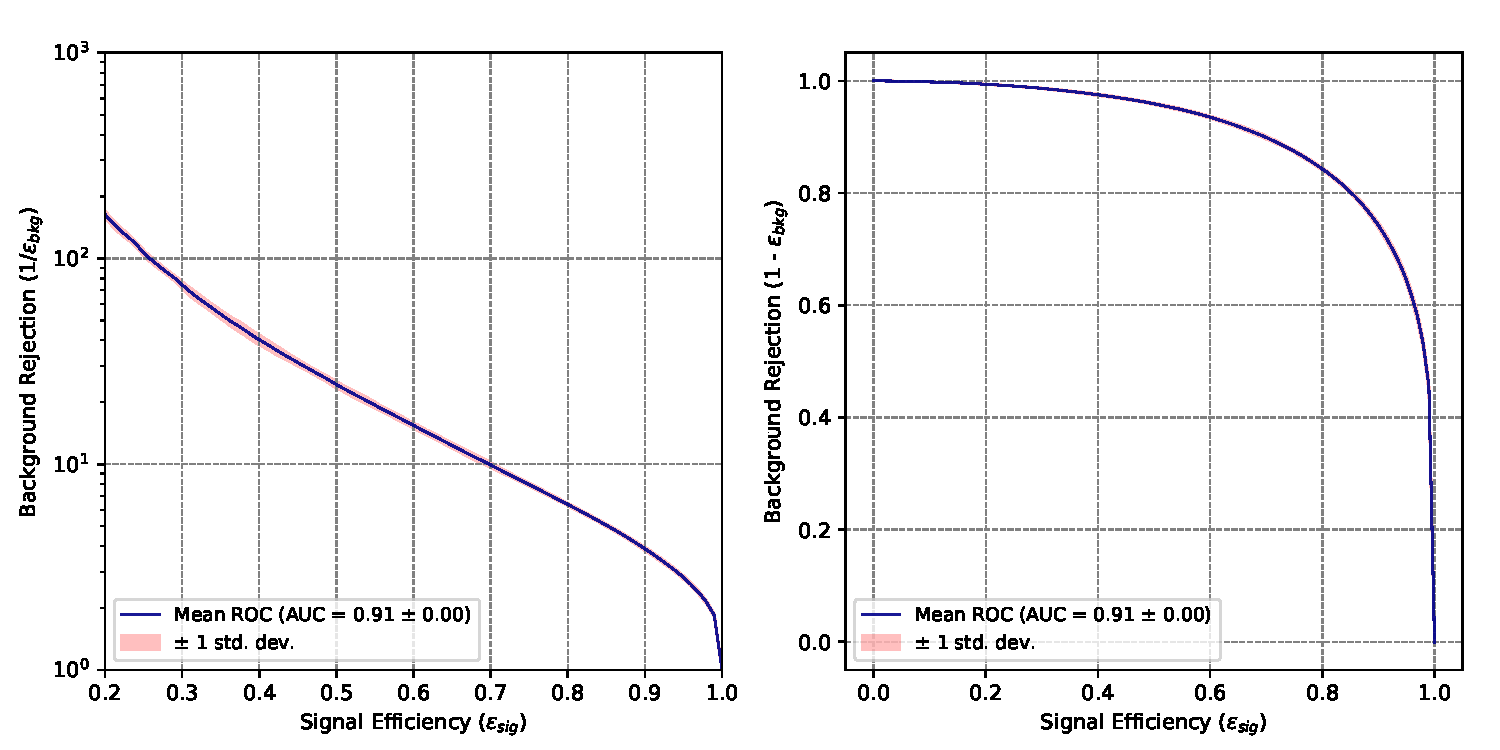
\includegraphics[width=0.6\textwidth]{figures/VH/VH_kfold_roc_ova_zdep.pdf}\label{fig:vh_ova_zdep_roc}
  }
  \caption{ROC curves for the ANN performance in the \zdom{} SR\@. The curves are averaged over the five folds of the cross-validation, with the shaded area representing the standard deviation across folds. The curves demonstrate good performance due to the high (AUC) score.}\label{fig:vh_wh_zdep_roc}
\end{figure}

\begin{figure}[htp]
  \centering
  \subfloat[$WH$ node in \zdom{} SR]{
    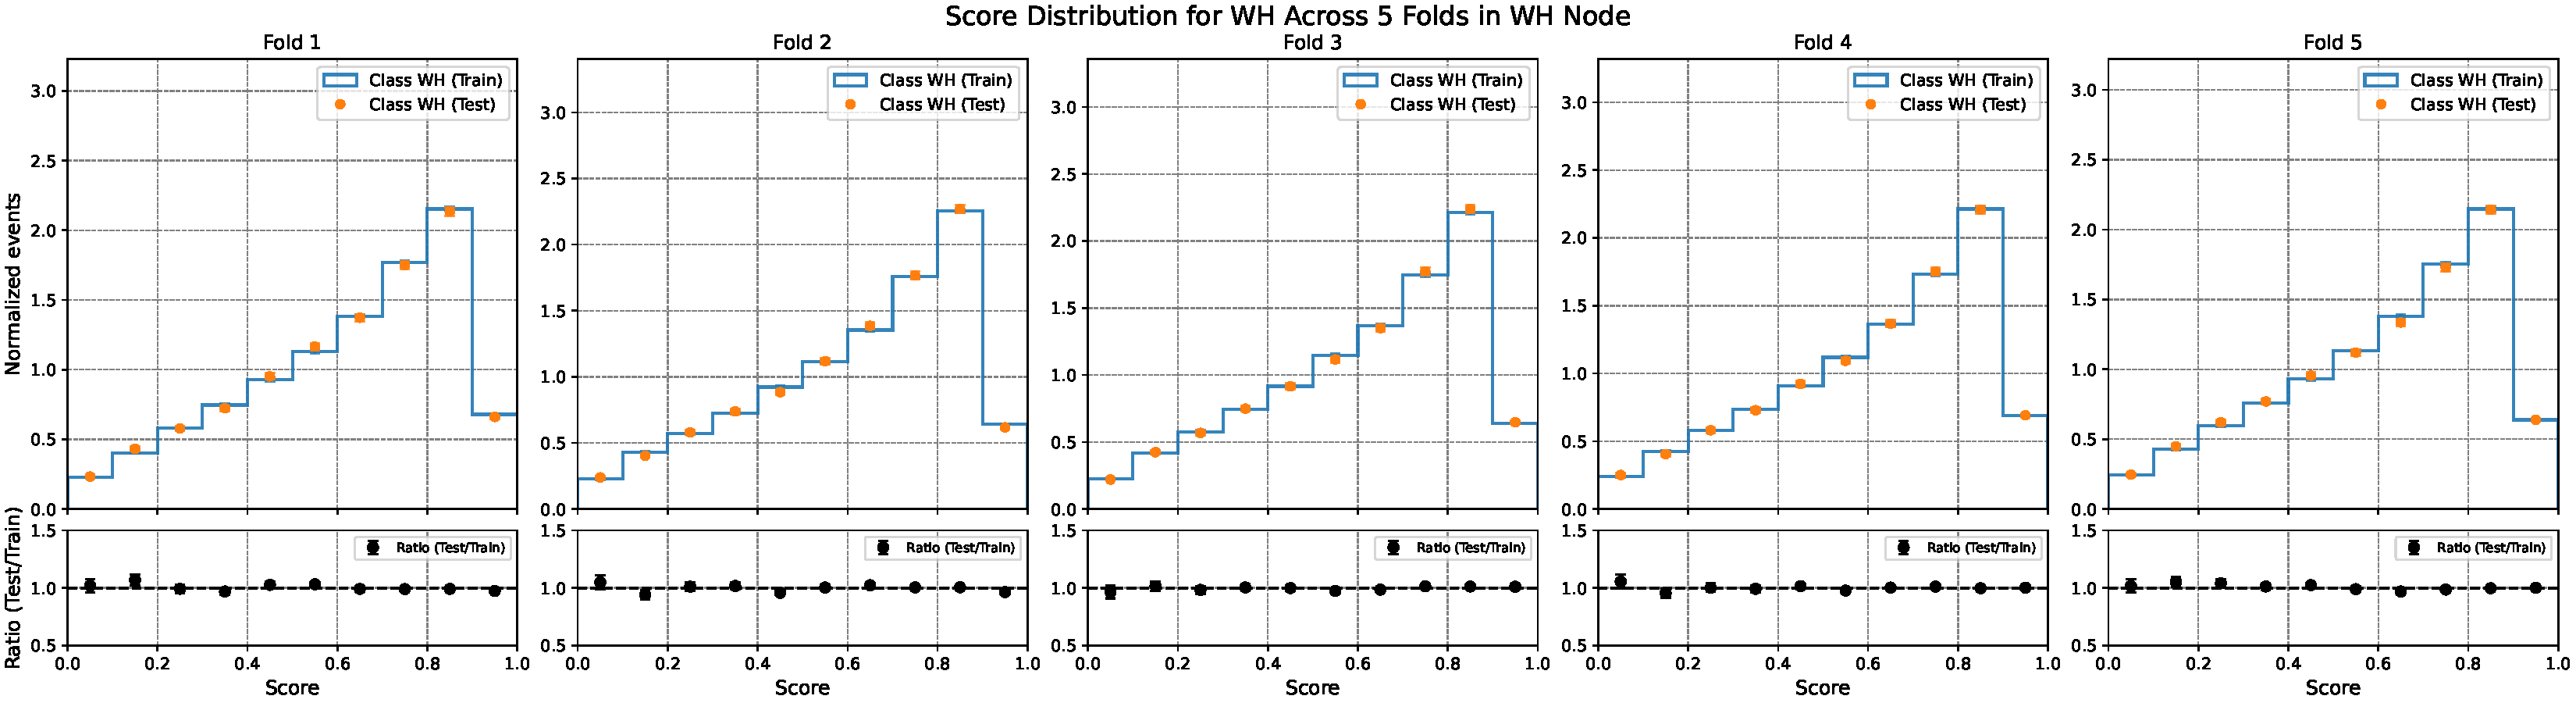
\includegraphics[width=1.1\textwidth]{figures/VH/VH_kfold_score_wh_zdom.pdf}\label{fig:vh_wh_zdom_kfold_scores1}
  }
  \hfill
  \subfloat[$WZ$ node in \zdom{} SR]{
    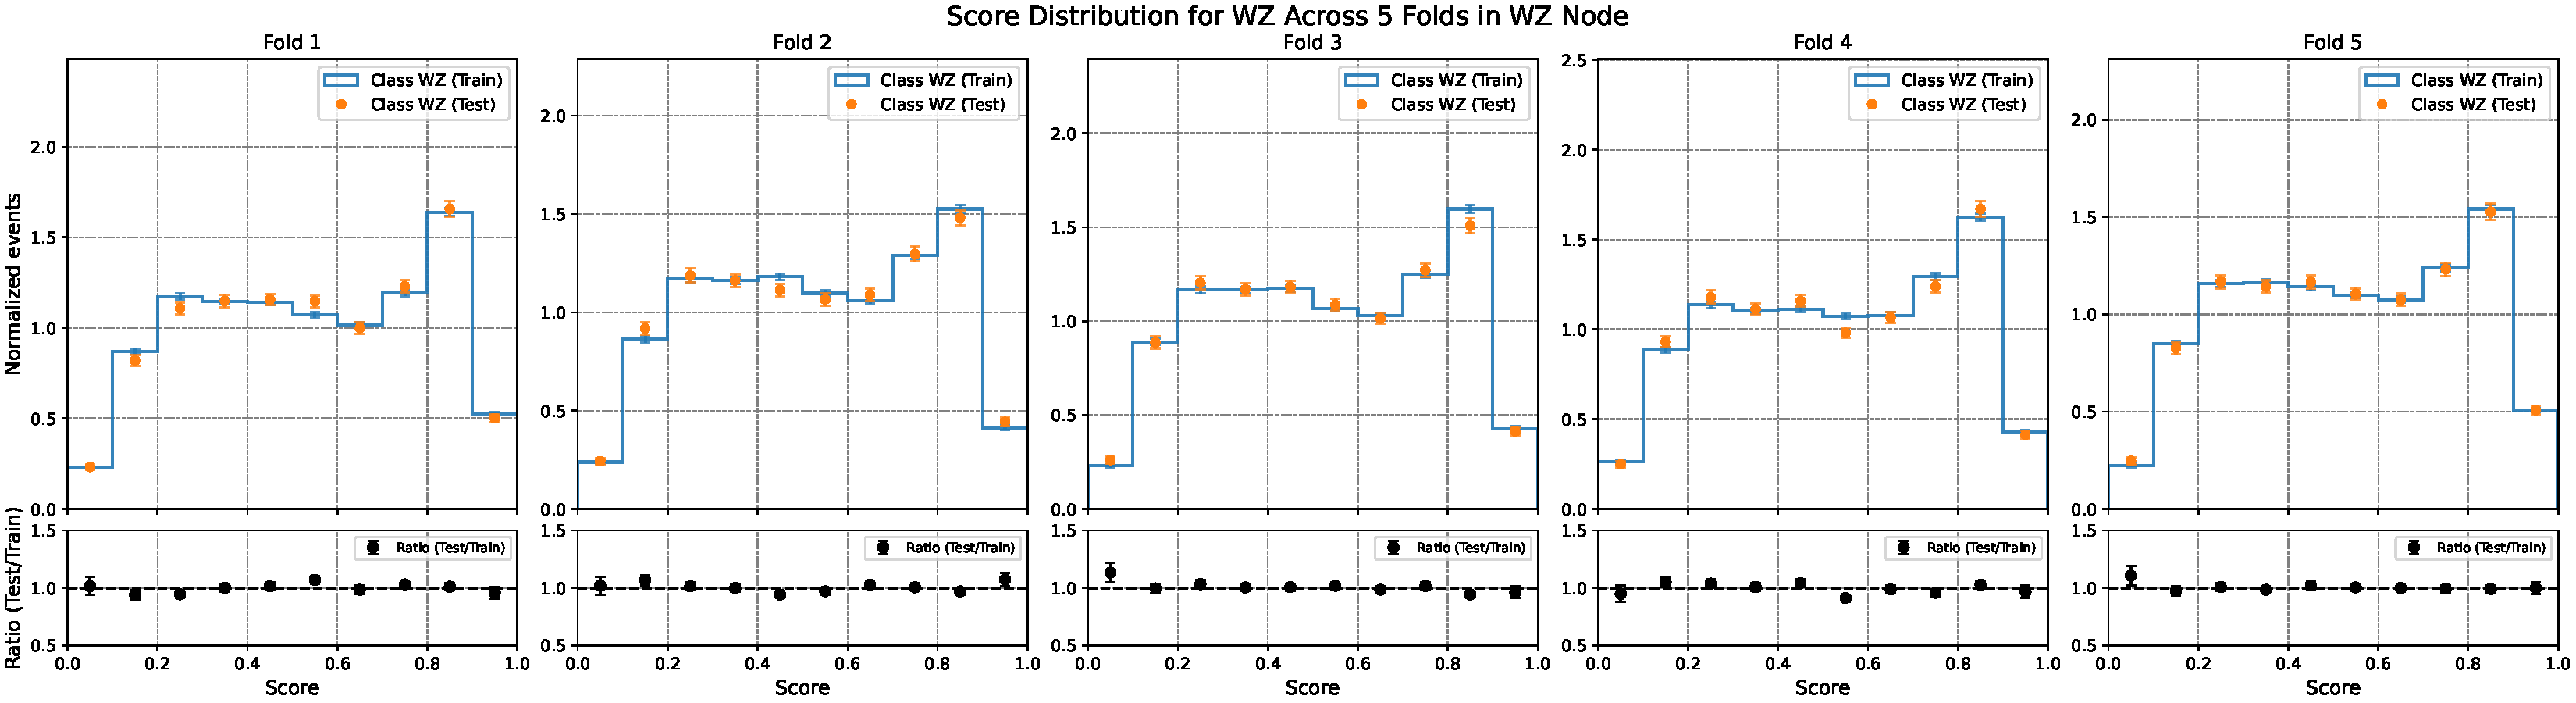
\includegraphics[width=1.1\textwidth]{figures/VH/VH_kfold_score_wz_zdom.pdf}\label{fig:vh_wh_wz_zdom_kfold_scores}
  }
  \hfill
  \subfloat[$ZZ$ node in \zdom{} SR]{
    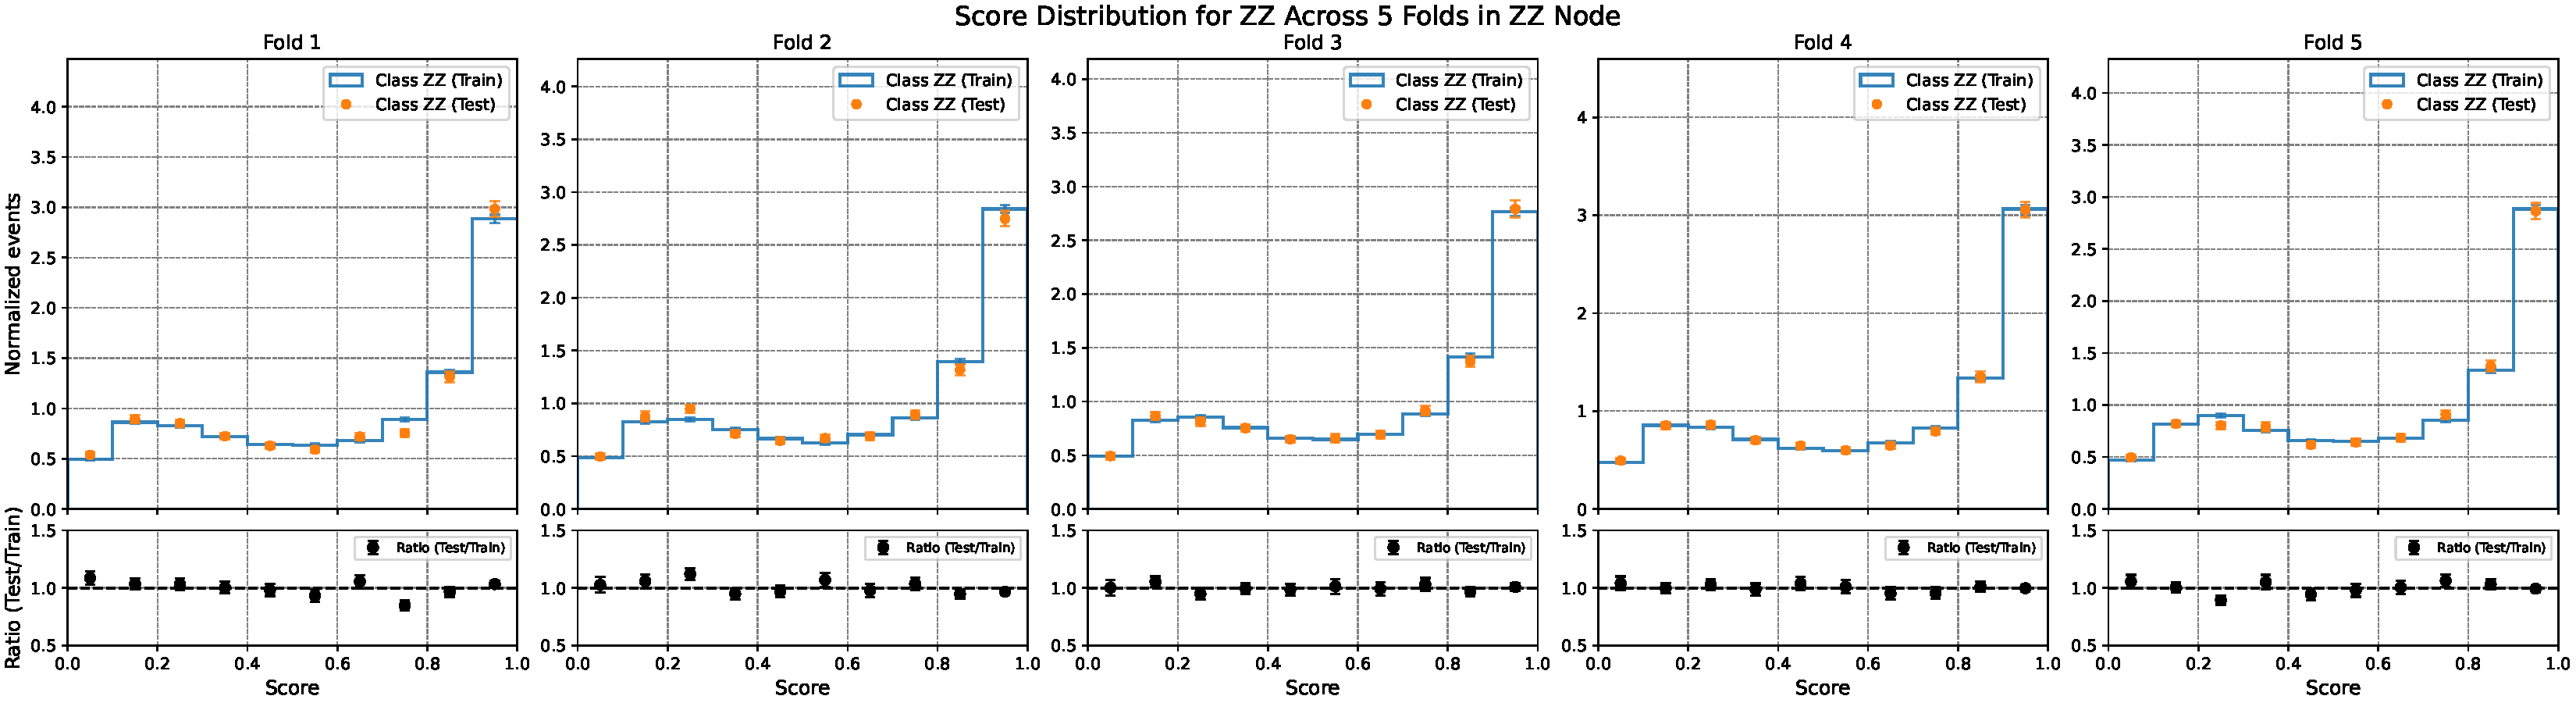
\includegraphics[width=1.1\textwidth]{figures/VH/VH_kfold_score_zz_zdom.pdf}\label{fig:vh_wh_zz_zdom_kfold_scores}
  }
  \caption{ANN score distributions for the \zdom{} SR\@. The distributions are shown for the $WH$, $WZ$, and $ZZ$ nodes across the five folds of the cross-validation. Each score distribution is plotted in the corresponding output node, hence all samples should peak in the high score bins.}\label{fig:vh_wh_zdom_kfold_scores}
\end{figure}


\begin{figure}[htp]
  \centering
  \subfloat[$WH$ node in \zdep{} SR]{
    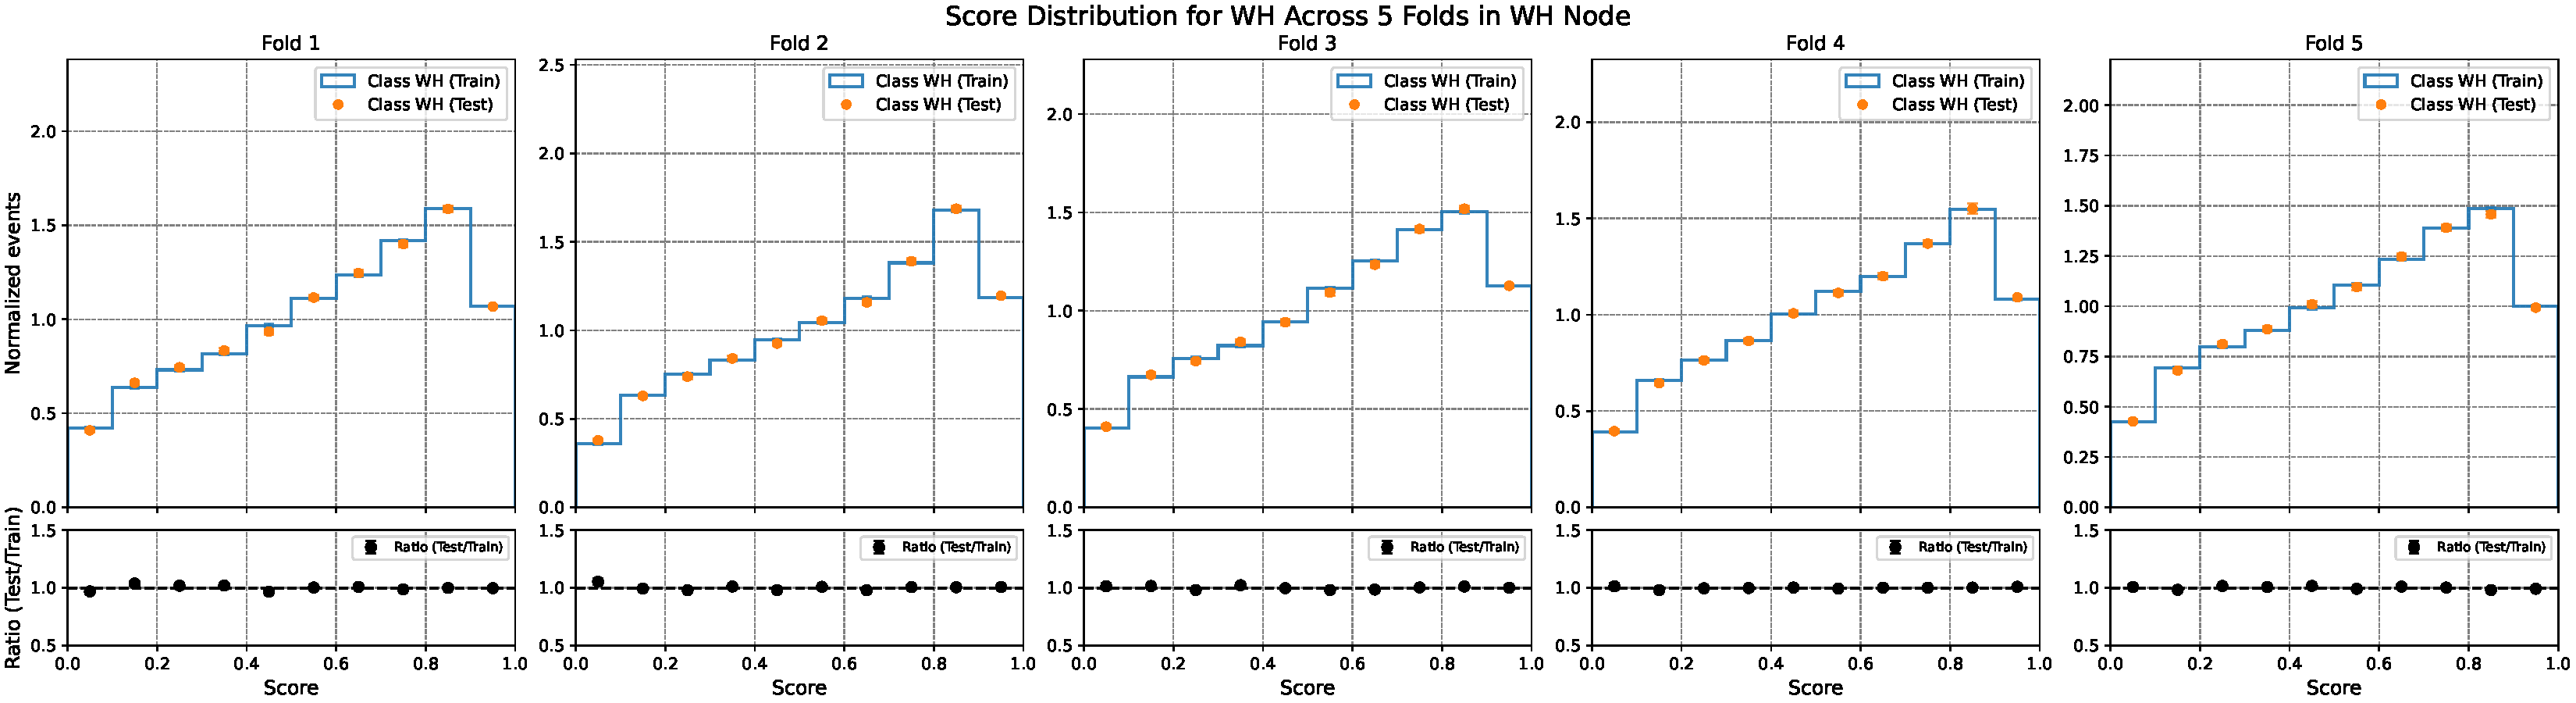
\includegraphics[width=1.05\textwidth]{figures/VH/VH_kfold_score_wh_zdep.pdf}\label{fig:vh_wh_zdep_kfold_scores1}
  }
  \hfill
  \subfloat[$WZ$ node in \zdep{} SR]{
    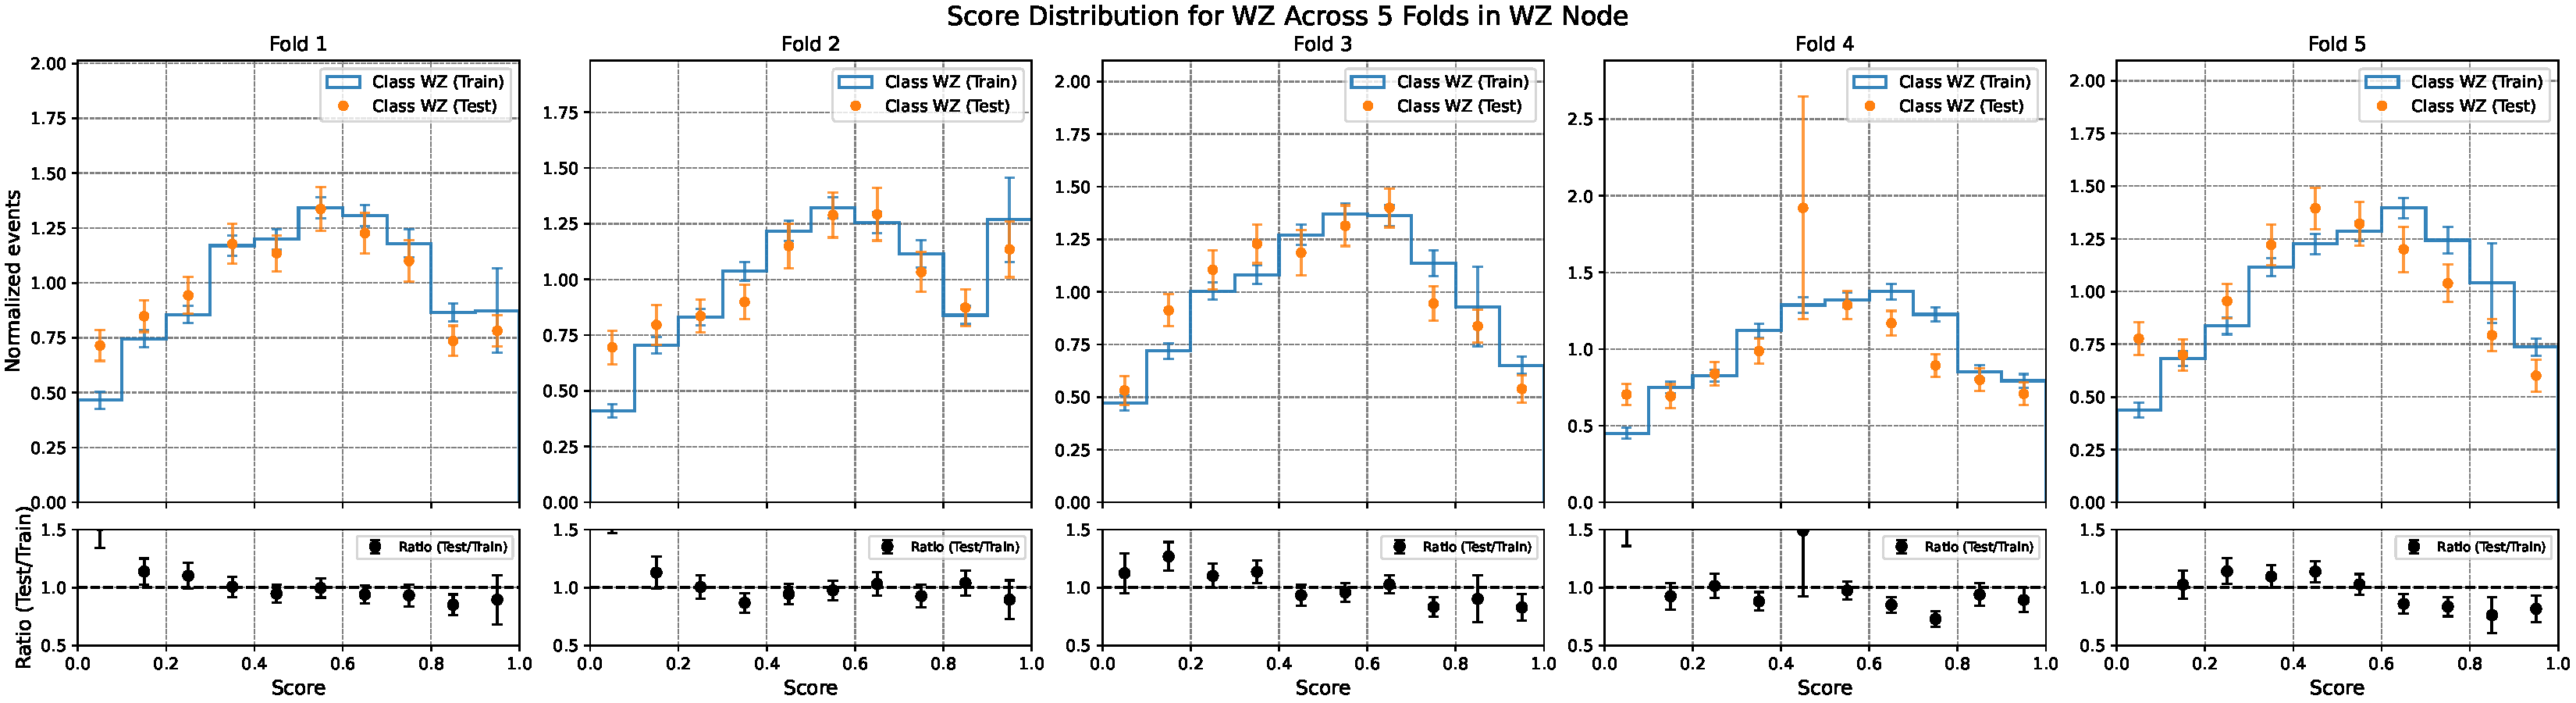
\includegraphics[width=1.05\textwidth]{figures/VH/VH_kfold_score_wz_zdep.pdf}\label{fig:vh_wh_wz_zdep_kfold_scores}
  }
  \hfill
  \subfloat[$WWW$ node in \zdep{} SR]{
    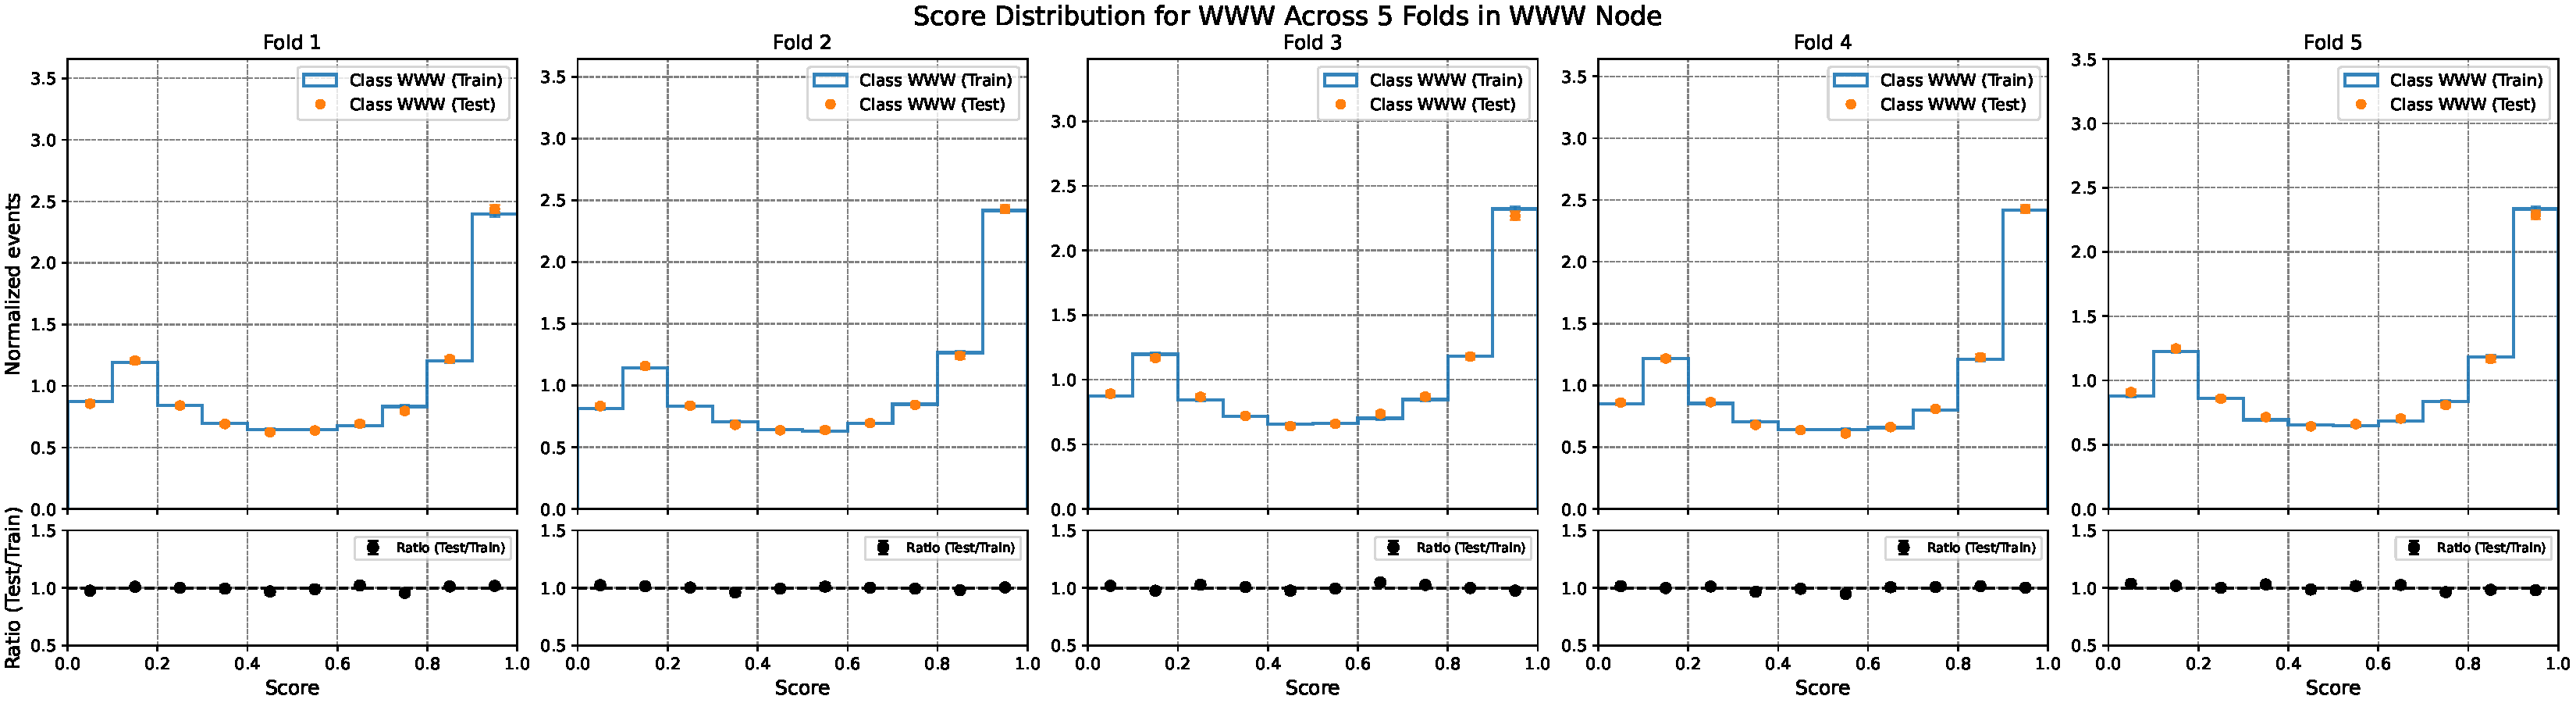
\includegraphics[width=1.05\textwidth]{figures/VH/VH_kfold_score_www_zdep.pdf}\label{fig:vh_wh_www_zdep_kfold_scores}
  }
  \hfill
  \subfloat[$t\bar{t}$ node in \zdep{} SR]{
    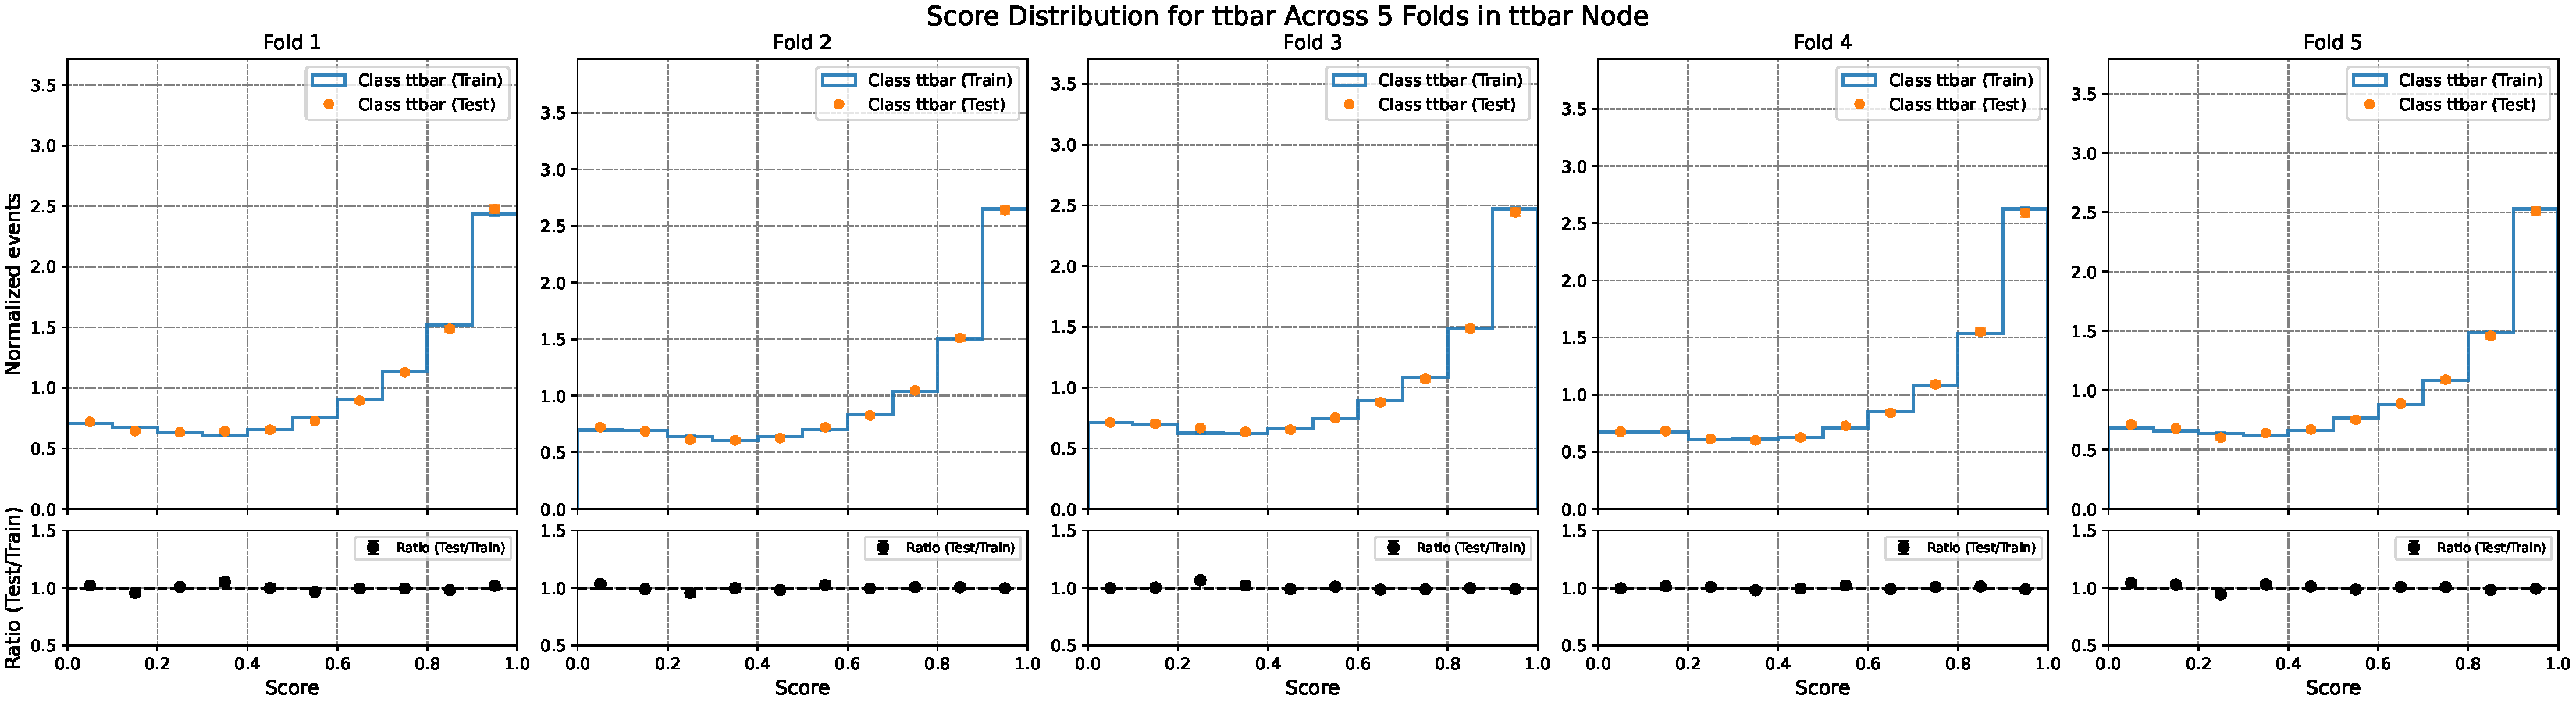
\includegraphics[width=1.05\textwidth]{figures/VH/VH_kfold_score_ttbar_zdep.pdf}\label{fig:vh_wh_ttbar_zdom_kfold_scores}
  }
  \caption{ANN score distributions for the \zdep{} SR\@. The distributions are shown for the $WH$, $WZ$, $WWW$, and $t\bar{t}$ nodes across the five folds of the cross-validation. Each score distribution is plotted in the corresponding output node, hence all samples should peak in the high score bins.}\label{fig:vh_wh_zdep_kfold_scores}
\end{figure}